\begin{itemize}
	\item A linked structure is one with a series of zero or more pieces of data, connected by pointers from one to another
	\begin{center}
		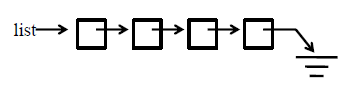
\includegraphics{sections/lec18/ll.png}
	\end{center}
	\item A list is another example of a container ADT
\end{itemize}

\subsection{List nodes}
\begin{itemize}
	\item We need to pick a concrete representation that stores a list as a dynamically created list of ``nodes''
\begin{lstlisting}[style=C++]
structNode {
	Node *next;
	int datum;
};
\end{lstlisting}
	\item Invariant:
	\begin{itemize}
		\item the datum field holds the integer datum of an element in the list
		\item Invariant: the next field points to the next Nodein the list, or 0 (AKA NULL) if no such Node exists
	\end{itemize}
	\item Resulting in the list's concrete implementation in the form of:
	\begin{center}
		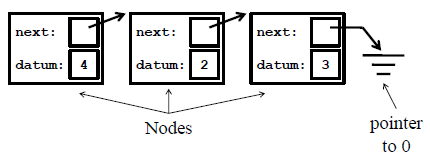
\includegraphics{sections/lec18/l1.png}
	\end{center}
\begin{lstlisting}[style=C++]
class IntList{
	//...
private:
	struct Node {
		Node *next;
		int datum;
	};
	Node *first;
};
\end{lstlisting}
	\item Representation invariant: \lstinline[style=C++]{first} points to the first node in the sequence of nodes representing this \lstinline[style=C++]{IntList}, or 0 if the list is empty
\end{itemize}

\subsection{Insert}
\begin{itemize}
	\item 
\begin{lstlisting}[style=C++]
void IntList::insertFront(int i) {
	Node *np= new Node;
	np->datum = i;
	np->next = first;
	first = np;
}
\end{lstlisting}
\begin{center}
	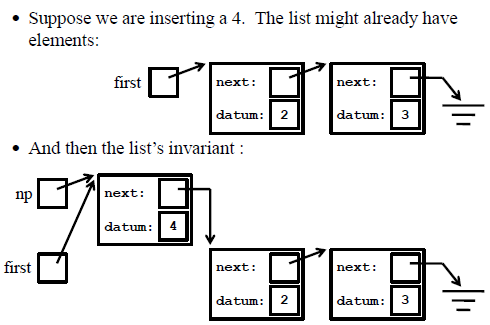
\includegraphics{sections/lec18/front.png}
\end{center}
\end{itemize}

\subsection{Implementing removeFront()}
\begin{itemize}
	\item If we are removing this first node, we must delete it to avoid a memory leak
	\item Unfortunately, we can't delete it before advancing the first pointer
\begin{lstlisting}[style=C++]
int IntList::removeFront() {
	assert(!isEmpty());
	Node *victim = first;
	first = first->next;
	int result = victim->datum;
	delete victim; victim=0;
	return result;
}	
\end{lstlisting}
\end{itemize}

\subsection{Implementing insertBack()}
\begin{itemize}
	\item Adding a member variable to point to the last item in a list, allows for trivial insert back
\begin{lstlisting}[style=C++]
void IntList::insertBack(inti) {
	Node *np= new Node;
	np->datum = i;
	np->next = 0;
	if (isEmpty()) {
		first = last = np;
	} else {
		last->next = np;
		last = np;
	}
}
\end{lstlisting}
\begin{center}
	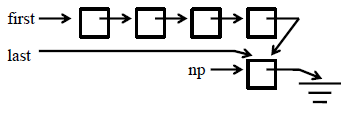
\includegraphics{sections/lec18/back.png}
\end{center}
	\item Removing from back is expensive because you must find the previous to last node: $\O{n}$
\end{itemize}

\subsection{Singly linked vs. doubly linked lists}
\begin{itemize}
	\item To make removal from the end efficient, as well, we have to have a doubly-linked list, so we can go forward and backward.
	\item In our new representation, a node is:
\begin{lstlisting}[style=C++]
structNode {
	Node *next;
	Node *prev;
	int datum;
}
\end{lstlisting}
	\item e.g., $[2, 3]$
\begin{center}
	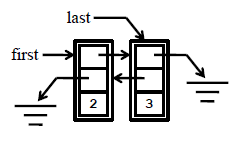
\includegraphics{sections/lec18/dl.png}
\end{center}
\end{itemize}